\documentclass[tikz,border=0pt]{standalone}
\usepackage[T1]{fontenc}
\usepackage[scaled=1.0]{helvet}
\usepackage{amsmath,amssymb,bm,graphicx}
\usepackage{xcolor}
\usetikzlibrary{arrows.meta,calc,positioning}

% GraphPad Prism-inspired publication styling:
% Helvetica-like sans serif, bold hierarchy, strong uniform strokes,
% high contrast, restrained accent colors, 16:9 edge-to-edge canvas.
\definecolor{ink}{HTML}{1E2B36}
\definecolor{outline}{HTML}{6D8292}
\definecolor{navy}{HTML}{163A57}
\definecolor{blue}{HTML}{176B99}
\definecolor{teal}{HTML}{007C79}
\definecolor{ice}{HTML}{F1F7FB}
\definecolor{mint}{HTML}{EDF8F6}
\definecolor{goldA}{HTML}{C88700}
\definecolor{paleGold}{HTML}{FFF4D6}
\definecolor{coralA}{HTML}{C4514B}
\definecolor{paleCoral}{HTML}{FFF0EE}
\definecolor{violetA}{HTML}{6651A8}
\definecolor{paleViolet}{HTML}{F3F0FB}
\definecolor{orangeA}{HTML}{BD5C00}
\definecolor{paleOrange}{HTML}{FFF3E6}

% All figure typography is explicit: consistent weights, not auto-scaled.
\newcommand{\StageTitle}[1]{{\bfseries\fontsize{12.8}{15}\selectfont #1}}
\newcommand{\StageBody}[1]{{\mdseries\fontsize{12.5}{16}\selectfont #1}}
\newcommand{\StageEmphasis}[1]{{\bfseries\fontsize{13.8}{16}\selectfont #1}}
\newcommand{\MetricTitle}[1]{{\bfseries\fontsize{12.7}{15.2}\selectfont #1}}
\newcommand{\MetricValue}[1]{{\bfseries\fontsize{25}{28}\selectfont #1}}
\newcommand{\MetricSmallValue}[1]{{\bfseries\fontsize{22}{26}\selectfont #1}}
\newcommand{\MetricUnits}[1]{{\mdseries\fontsize{11.8}{14}\selectfont #1}}
\newcommand{\FooterMetric}[1]{{\sffamily\fontsize{10.7}{12.9}\selectfont #1}}

\begin{document}
\begin{tikzpicture}[
  x=0.4in,y=0.4in,
  font=\sffamily,
  stage/.style={draw=outline,fill=white,rounded corners=2.6pt,
    line width=1.5pt,text=ink,align=center,
    text width=5.30cm,minimum height=3.82cm,
    inner xsep=5pt,inner ysep=5pt},
  keyblue/.style={stage,draw=blue,line width=2pt,fill=ice},
  keyteal/.style={stage,draw=teal,line width=2pt,fill=mint},
  naturalstage/.style={stage,draw=goldA,fill=paleGold},
  proteinstage/.style={stage,draw=coralA,fill=paleCoral},
  prepstage/.style={stage,draw=blue,fill=ice},
  validationstage/.style={stage,draw=violetA,fill=paleViolet},
  hitstage/.style={stage,draw=violetA,fill=paleViolet},
  analysisstage/.style={stage,draw=teal,fill=mint},
  energystage/.style={stage,draw=orangeA,fill=paleOrange},
  graphframe/.style={draw=outline,fill=white,rounded corners=2.3pt,line width=1.35pt},
  arrow/.style={-{Stealth[length=3.1mm,width=2.3mm]},
    line width=1.6pt,draw=navy,rounded corners=2.3pt}
]
  % Bounding box is exactly 16 x 9 inches; no title, caption, or margins.
  \useasboundingbox (0,0) rectangle (40,22.5);
  \path[fill=white] (0,0) rectangle (40,22.5);

  % --------------------- BOTANICAL SOURCE PANEL ---------------------
  \filldraw[draw=goldA,line width=2.0pt,fill=paleGold,rounded corners=3pt]
      (0.42,10.68) rectangle (8.54,22.05);
  \node[anchor=center,text=navy,align=center,
    font=\sffamily\bfseries\fontsize{14.9}{17.4}\selectfont]
      at (4.48,21.42) {BOTANICAL SOURCE};

  \filldraw[draw=goldA,line width=1.35pt,fill=white,rounded corners=2pt]
      (0.86,13.52) rectangle (4.38,20.58);
  \filldraw[draw=goldA,line width=1.35pt,fill=white,rounded corners=2pt]
      (4.59,13.52) rectangle (8.11,20.58);
  \node[inner sep=0pt] at (2.62,17.05)
      {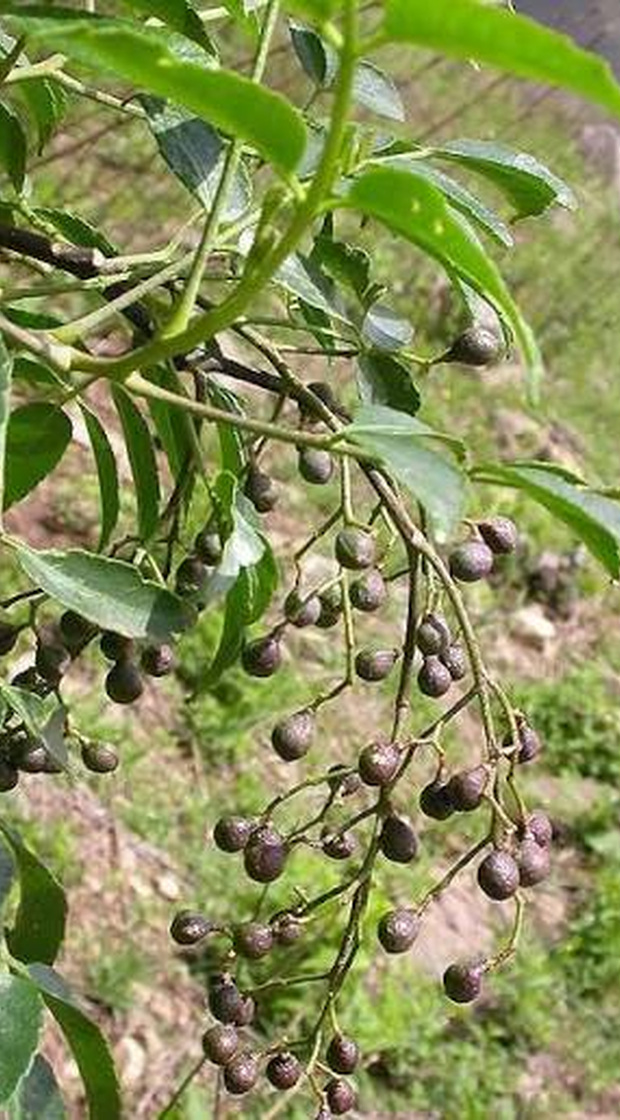
\includegraphics[width=1.345in,height=2.695in]{assets/botanical_fruits.jpg}};
  \node[inner sep=0pt] at (6.35,17.05)
      {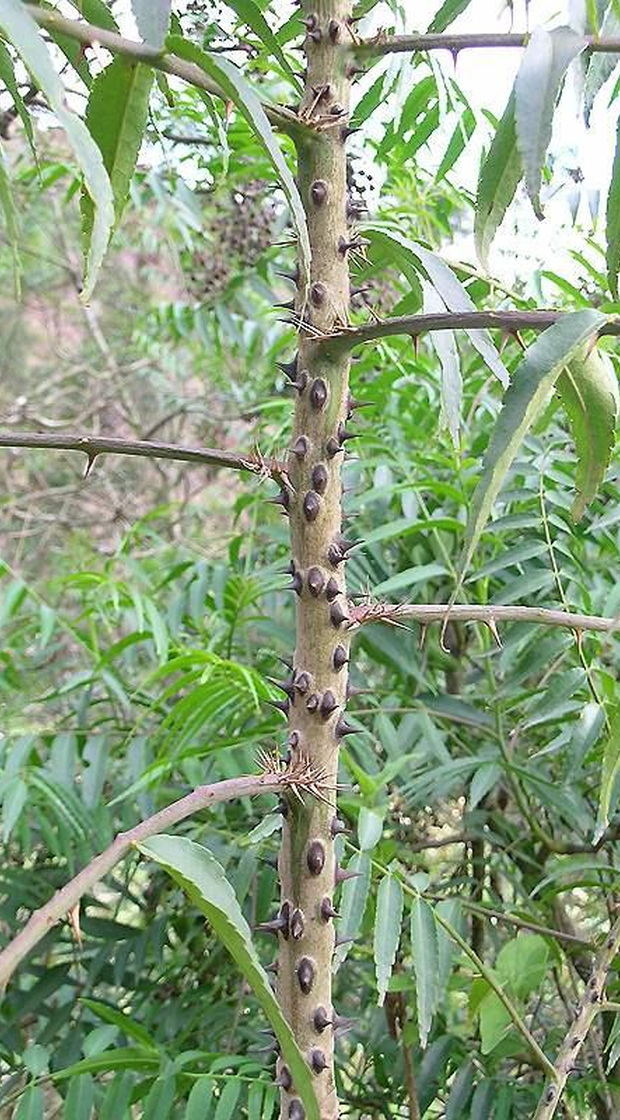
\includegraphics[width=1.345in,height=2.695in]{assets/botanical_stem.jpg}};

  \node[align=center,anchor=center,text=navy,
    font=\sffamily\fontsize{12.8}{15.2}\selectfont]
      at (4.48,12.36) {\textit{Zanthoxylum chalybeum}};
  \node[align=center,anchor=center,text=ink,
    font=\sffamily\bfseries\fontsize{12.3}{15}\selectfont]
      at (4.48,11.37) {15 natural products};

  % --------------------- WORKFLOW ROWS ---------------------
  \node[prepstage] (ligprep) at (12.08,19.35)
    {\StageTitle{LIGAND PREPARATION}\\[11pt]
     \StageBody{Protonation at pH 5.0}};

  \node[keyblue,fill=blue,text=white,draw=blue] (docking) at (19.93,19.35)
    {\StageTitle{MOLECULAR DOCKING}\\[10pt]
     \StageBody{AutoDock Vina}\\[5pt]
     \StageBody{15 natural products}};

  \node[hitstage] (hits) at (27.73,19.35)
    {\StageTitle{TOP DOCKING HITS}\\[7pt]
     \MetricUnits{Docking score (kcal/mol)}\\[9pt]
     \StageBody{THL: \textbf{--8.411}}\\[5pt]
     \StageBody{SES: \textbf{--8.369}}\\[5pt]
     \StageBody{NCH: \textbf{--8.138}}};

  \node[keyteal,fill=teal,text=white,draw=teal] (md) at (35.48,19.35)
    {\StageTitle{MOLECULAR DYNAMICS}\\[10pt]
     \StageEmphasis{400 ns per system}\\[7pt]
     \StageBody{Apo PMII $\mid$ R37 $\mid$ THL}\\[5pt]
     \StageBody{SES $\mid$ NCH}};

  \node[proteinstage] (receptor) at (12.08,13.62)
    {\StageTitle{RECEPTOR PREPARATION}\\[8pt]
     \StageBody{Plasmepsin II (PMII)}\\[5pt]
     \StageBody{Protonation at pH 5.0}};

  \node[validationstage] (validation) at (19.93,13.62)
    {\StageTitle{DOCKING VALIDATION}\\[10pt]
     \StageBody{R37 redocking}};

  \node[analysisstage] (trajectory) at (27.73,13.62)
    {\StageTitle{TRAJECTORY ANALYSIS}\\[8pt]
     \StageBody{RMSD, RMSF, $R_g$, SASA}\\[6pt]
     \StageBody{Binding-site retention}\\[5pt]
     \StageBody{Hydrogen-bond dynamics}};

  \node[energystage] (mmpbsa) at (35.48,13.62)
    {\StageTitle{MM/PBSA ANALYSIS}\\[8pt]
     \StageBody{Final 200 ns (200--400 ns)}\\[6pt]
     \StageBody{200 snapshots per complex}\\[5pt]
     \StageBody{Binding-energy estimation}};

  % Connectors
  \draw[arrow] (8.54,19.35) -- (ligprep.west);
  \draw[arrow] (ligprep.east) -- (docking.west);
  \draw[arrow] (docking.east) -- (hits.west);
  \draw[arrow] (hits.east) -- (md.west);
  \draw[arrow] (receptor.east) -- (validation.west);
  \draw[arrow] (validation.north) -- (docking.south);
  \draw[arrow] (md.south) -- (35.48,16.38) -- (35.48,16.38) -- (mmpbsa.north);
  \draw[arrow] (md.south) -- (35.48,16.38) -| (trajectory.north);

  % --------------------- PRIORITIZED RESULT PANEL ----------------
  \filldraw[draw=blue,line width=2.1pt,fill=ice,
    rounded corners=3.2pt]
    (0.35,0.35) rectangle (39.65,10.32);

  \node[align=center,anchor=center,text=navy,
    font=\sffamily\bfseries\fontsize{18.5}{22}\selectfont]
    at (20,9.18)
    {LEAD CANDIDATE: 3,20,28-TRIHYDROXYLUPANE (THL)};
  \draw[blue,line width=1.45pt]
    (0.82,8.10) -- (39.18,8.10);

  % arrows to panel edge only
  \draw[arrow] (trajectory.south) -- (27.73,10.45);
  \draw[arrow] (mmpbsa.south) -- (35.48,10.45);

  % Graph labels
  \node[anchor=center,text=navy,font=\sffamily\bfseries\fontsize{11.8}{13.8}\selectfont]
    at (10.25,7.42) {H-BOND COUNT DYNAMICS (400 ns)};
  \node[anchor=center,text=navy,font=\sffamily\bfseries\fontsize{11.8}{13.8}\selectfont]
    at (29.75,7.42) {RESIDUE-SPECIFIC H-BOND OCCUPANCY};

  % Left graph frame
  \filldraw[graphframe,draw=violetA]
    (1.05,1.98) rectangle (19.45,7.05);
  \begin{scope}
    \clip[rounded corners=2.0pt] (1.18,2.11) rectangle (19.32,6.92);
    \node[anchor=center] at (10.25,4.515)
      {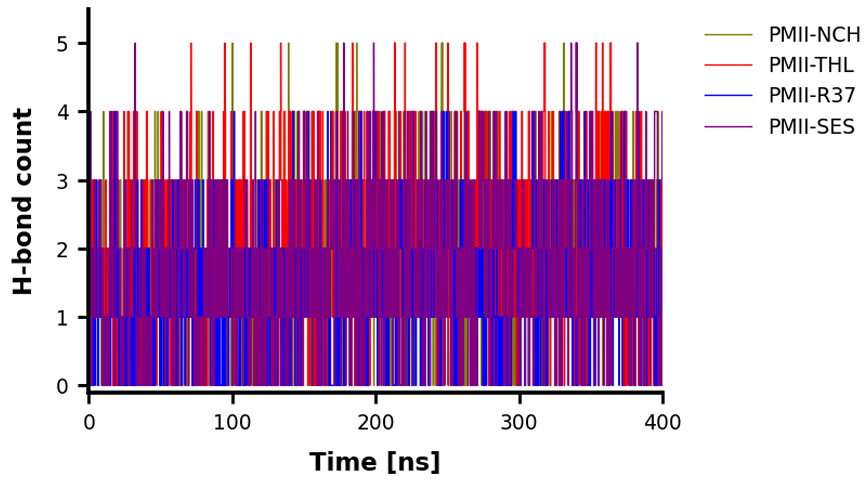
\includegraphics[width=18.14cm,height=4.81cm]{assets/hbond_count.png}};
  \end{scope}

  % Right graph frame
  \filldraw[graphframe,draw=goldA]
    (20.55,1.98) rectangle (38.95,7.05);
  \begin{scope}
    \clip[rounded corners=2.0pt] (20.68,2.11) rectangle (38.82,6.92);
    \node[anchor=center] at (29.75,4.515)
      {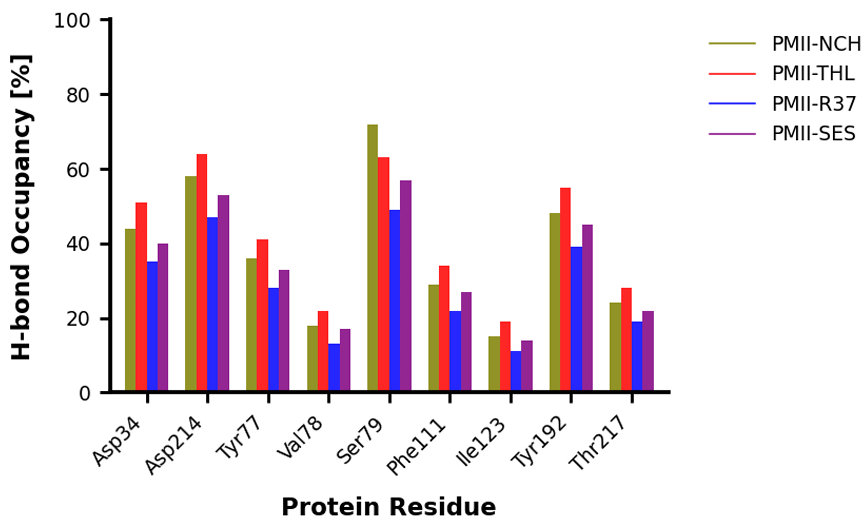
\includegraphics[width=18.14cm,height=4.81cm]{assets/hbond_occupancy.png}};
  \end{scope}

  % compact evidence strip
  \node[align=center,text=ink,font=\sffamily\fontsize{10.5}{12.8}\selectfont]
    at (20,1.00)
    {Docking score: \textbf{--8.411} kcal/mol \quad $\bullet$ \quad Contact retention: \textbf{82.8\%} \quad $\bullet$ \quad Mean H-bonds: \textbf{1.93} \\
     Asp34 occupancy: \textbf{51\%} \quad $\bullet$ \quad Asp214 occupancy: \textbf{64\%} \quad $\bullet$ \quad MM/PBSA: \textbf{--47.38 $\pm$ 2.72} kcal/mol};
\end{tikzpicture}
\end{document}